\documentclass[12pt, a4paper]{report}

% Packages :

\usepackage[french]{babel}
\usepackage[utf8]{inputenc}
\usepackage[T1]{fontenc}
\usepackage[pdftex, pdfauthor={Bacomathiques}]{hyperref}
\usepackage{sectsty}
\usepackage[explicit]{titlesec}
\usepackage{xcolor}
\usepackage{amsmath}
\usepackage{amssymb}
\usepackage{amsthm}
\usepackage{fourier}
\usepackage{titlesec}
\usepackage{fancyhdr}
\usepackage{catchfilebetweentags}
\usepackage[french, capitalise, noabbrev]{cleveref}
\usepackage[fit, breakall]{truncate}
\usepackage[margin=3cm]{geometry}
\usepackage{tocloft}
\usepackage{tikz}
\usepackage{tocloft}
\usepackage{microtype}
\usepackage{listings}
\usepackage{tabularx}
\usepackage{calc}
\usepackage[export]{adjustbox}
\usepackage[most]{tcolorbox}
\usepackage{standalone}
\usepackage{xlop}
\usepackage{etoolbox}
\usepackage{environ}

\usetikzlibrary{arrows.meta}
\usetikzlibrary{trees}

% Paramètres :

\author{Bacomathiques}
\definecolor{graphe}{HTML}{93c9ff}
\setcounter{MaxMatrixCols}{12}
\setlength{\parindent}{0pt}
\setlength{\fboxsep}{0pt}
%\pdfsuppresswarningpagegroup=1

% Code :

\lstdefinestyle{style}{
	backgroundcolor=\color{white},
	commentstyle=\em\color[HTML]{999988},
	keywordstyle=\bfseries,
	identifierstyle=\normalfont,
	stringstyle=\color[rgb]{0.87, 0.07, 0.27},
	basicstyle=\ttfamily\color{black},
	breakatwhitespace=false,
	breaklines=true,
	captionpos=b,
	keepspaces=true,
	numbers=left,
	numbersep=5pt,
	showspaces=false,
	showstringspaces=false,
	showtabs=false,
	tabsize=2,
	numbers=none
}

\lstset{style=style}
\lstset{
	literate=
	{á}{{\'a}}1
	{à}{{\`a}}1
	{ã}{{\~a}}1
	{é}{{\'e}}1
	{ê}{{\^e}}1
	{í}{{\'i}}1
	{ó}{{\'o}}1
	{õ}{{\~o}}1
	{ú}{{\'u}}1
	{ü}{{\"u}}1
	{ç}{{\c{c}}}1
}

\lstset{
	framextopmargin=10pt,
	framexrightmargin=10pt,
	framexbottommargin=10pt,
	framexleftmargin=10pt,
	xleftmargin=10pt,
	xrightmargin=10pt,
}

% Couleurs :

\definecolor{title}{HTML}{912c21}
\definecolor{section}{HTML}{1c567d}
\definecolor{subsection}{HTML}{2980b9}

\definecolor{rule}{HTML}{c4c4c4}

\definecolor{formula}{HTML}{ebf3fb}
\definecolor{formula-left}{HTML}{3583d6}

\definecolor{tip}{HTML}{dcf3d8}
\definecolor{tip-left}{HTML}{26a65b}

\definecolor{demonstration}{HTML}{fff8de}
\definecolor{demonstration-left}{HTML}{f1c40f}

\definecolor{exercise}{HTML}{e0f2f1}
\definecolor{exercise-left}{HTML}{009688}

\definecolor{correction}{HTML}{e0f7fa}
\definecolor{correction-left}{HTML}{00bcd4}

\definecolor{toc}{HTML}{fceae9}
\definecolor{toc-left}{HTML}{e74c3c}
\definecolor{toc-dark}{HTML}{87281f}

% Titres :

\renewcommand{\thesection}{\Roman{section} - }
\renewcommand{\thesubsection}{\arabic{subsection}. }

\newcommand{\sectionstyle}{\normalfont\LARGE\bfseries\color{section}}
\titleformat{\section}{\sectionstyle}{\thesection #1}{0pt}{}
\titleformat{name=\section, numberless}{\sectionstyle}{#1}{0pt}{}

\newcommand{\subsectionstyle}{\normalfont\Large\bfseries\color{subsection}}
\titleformat{\subsection}{\subsectionstyle}{\thesubsection #1}{0pt}{}
\titleformat{name=\subsection, numberless}{\subsectionstyle}{#1}{0pt}{}

\titlelabel{\thetitle\ }

% Table des matières :

\addto\captionsfrench{\renewcommand\contentsname{}}
\renewcommand{\cftsecpagefont}{\color{toc-dark}}
\renewcommand{\cftsubsecpagefont}{\color{toc-dark}}
\renewcommand{\cftsecleader}{\cftdotfill{\cftdotsep}}
\renewcommand{\cftsecfont}{\bfseries}
\renewcommand{\cftsecpagefont}{\bfseries\color{toc-dark}}
\setlength{\cftbeforetoctitleskip}{0pt}
\setlength{\cftaftertoctitleskip}{0pt}
\setlength{\cftsecindent}{0pt}
\setlength{\cftsubsecindent}{20pt}
\setlength{\cftsubsecnumwidth}{20pt}

% Commandes :

\newcommand{\newpar}{\\[\medskipamount]}
\newcommand{\lesson}[3]{%
	\newcommand{\level}{#1}%
	\newcommand{\id}{#2}%
	\hypersetup{pdftitle={#3}}
	\begin{center}%
		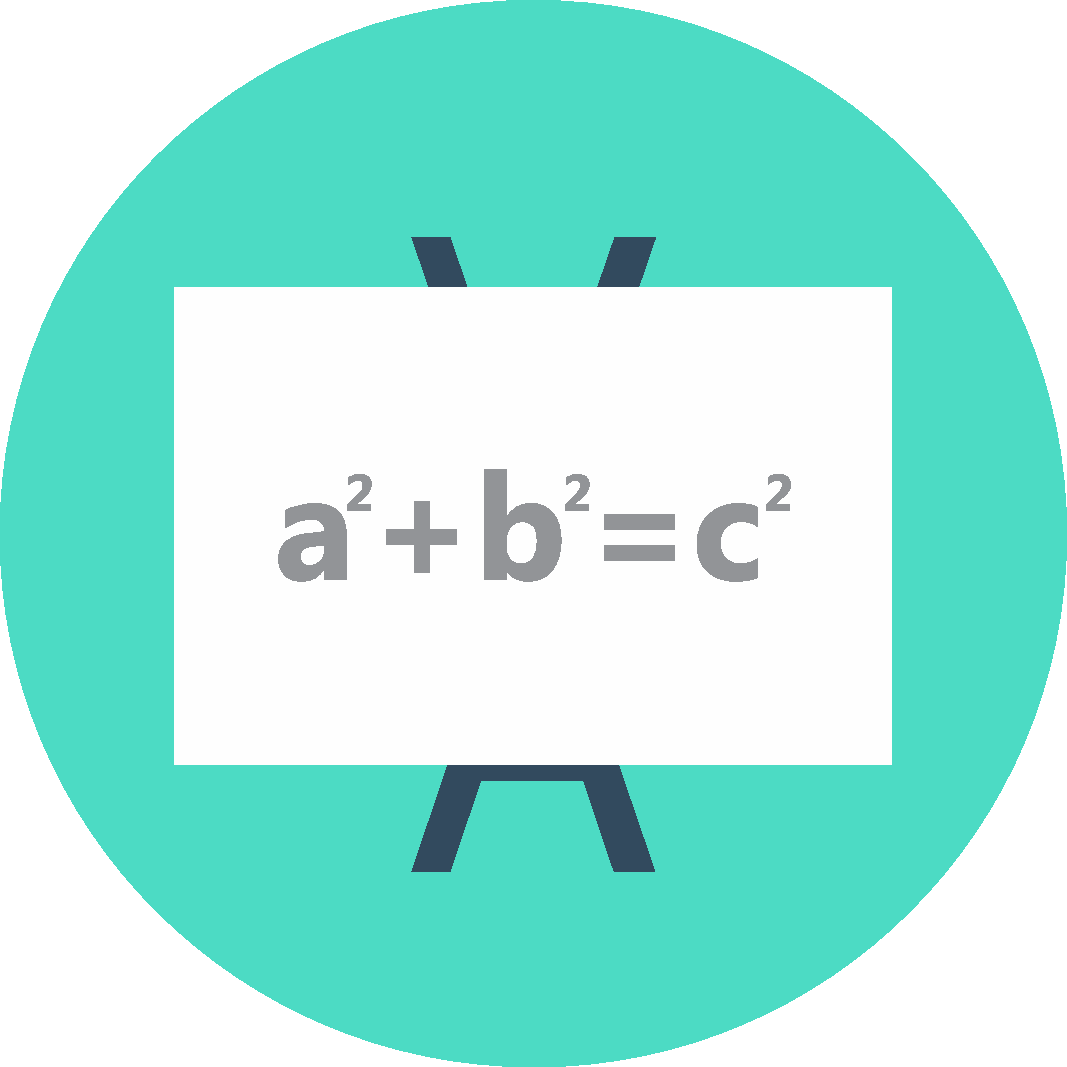
\includegraphics[width=150px]{\imagespath/bacomathiques}%
		
		\vspace{30pt}%
		{\Huge\color{title} #3}%
		
		\vspace{10pt}%
		{Bacomathiques --- \href{https://bacomathiqu.es/cours/#1/#2}{\color{section} https://bacomathiqu.es}}%
		
		\vspace{20pt}%
	\end{center}%
	\begin{toc}
		\tableofcontents%
	\end{toc}
	\thispagestyle{empty}%
	\newpage%
	\setcounter{page}{1}%
}
\newcommand{\imagespath}{../../images}
\newcommand{\lessonimagespath}{\imagespath/lessons/\level/\id/}
\newcommand{\includelatexpicture}[2][\textwidth - 100pt]{%
	\begin{center}%
		\resizebox{#1}{!}{%
			\input{\lessonimagespath#2}%
		}%
	\end{center}%
	\medskip%
}
\newcommand{\includeimage}[1]{%
	\begin{center}%
		\includegraphics{\lessonimagespath#1}%
	\end{center}%
	\medskip%
}
\newcommand{\includerepresentation}[1]{%
	\begin{center}%
		\setlength{\fboxrule}{0.5pt}%
		\href{https://www.geogebra.org/m/#1}{\includegraphics[width=\textwidth-1pt,fbox]{\lessonimagespath#1}}%
	\end{center}%
}
\newcommand{\floor}[1]{\lfloor #1 \rfloor}

\makeatletter
\newcommand\inputcontent{\@ifstar{\inputcontent@star}{\inputcontent@nostar}}
\newcommand{\inputcontent@star}[1]{%
	\ExecuteMetaData[#1]{content}%
}
\newcommand{\inputcontent@nostar}[1]{%
	\newpage%
	\inputcontent@star{#1}%
}
\makeatother

\let\oldsection\section
\renewcommand\section{\clearpage\oldsection}
\newcommand{\contentwidth}[1][medium]{}

% En-têtes :

\pagestyle{fancy}

\renewcommand{\sectionmark}[1]{\markboth{\thesection \ #1}{}}

\fancyhead[R]{\truncate{0.23\textwidth}{\color{title}\thepage}}
\fancyhead[L]{\truncate{0.73\textwidth}{\color{title}\leftmark}}
\fancyfoot[C]{\scriptsize \href{https://bacomathiqu.es/cours/\level/\id}{\texttt{bacomathiqu.es}}}

\makeatletter
\patchcmd{\f@nch@head}{\rlap}{\color{rule}\rlap}{}{}
\patchcmd{\headrule}{\hrule}{\color{rule}\hrule}{}{}
\makeatother

% Environnements :

\newenvironment{nosummary}{}{}
\newcommand{\tcolorboxtitle}[2]{\setlength{\fboxsep}{2.5pt}\hspace{-10pt}\colorbox{#1-left}{\hspace{8pt}\MakeUppercase{#2} \hspace{2pt} \includegraphics[height=0.8em]{\imagespath/bubbles/#1}\hspace{5pt}}}
\newcommand{\tcolorboxsubtitle}[2]{\ifstrempty{#2}{}{\textcolor{#1-left}{\large#2}\\[\medskipamount]}}
\tcbset{
	frame hidden,
	boxrule=0pt,
	boxsep=0pt,
	enlarge bottom by=8.5pt,
	enhanced jigsaw,
	boxed title style={sharp corners,boxrule=0pt,coltitle={white},titlerule=0pt},
	fonttitle=\fontsize{6pt}{6pt}\bfseries\boldmath,
	top=10pt,
	right=10pt,
	bottom=10pt,
	left=10pt,
	arc=0pt,
	outer arc=0pt,
}
\newtcolorbox{toc}[1][]{
	colback=toc,
	borderline west={3pt}{0pt}{toc-left},
	title=\tcolorboxtitle{toc}{Table des matières},
	colbacktitle=toc,
	before upper={\tcolorboxsubtitle{toc}{#1}}
}
\newtcolorbox{formula}[1][]{
	colback=formula,
	borderline west={3pt}{0pt}{formula-left},
	title=\tcolorboxtitle{formula}{À retenir},
	colbacktitle=formula,
	before upper={\tcolorboxsubtitle{formula}{#1}}
}
\newtcolorbox{tip}[1][]{
	colback=tip,
	borderline west={3pt}{0pt}{tip-left},
	title=\tcolorboxtitle{tip}{À lire},
	colbacktitle=tip,
	before upper={\tcolorboxsubtitle{tip}{#1}}
}
\newtcolorbox{demonstration}[1][]{
	colback=demonstration,
	borderline west={3pt}{0pt}{demonstration-left},
	title=\tcolorboxtitle{demonstration}{Démonstration},
	colbacktitle=demonstration,
	before upper={\tcolorboxsubtitle{demonstration}{#1}}
}

\NewEnviron{whitetabularx}[1]{%
	\renewcommand{\arraystretch}{2.5}
	\colorbox{white}{%
		\begin{tabularx}{\textwidth}{#1}%
			\BODY%
		\end{tabularx}%
	}%
}

% Longueurs :

\newlength{\espacetitreliste}
\setlength{\espacetitreliste}{-16pt}
\newcommand{\entretitreetliste}{\vspace{\espacetitreliste}}

\begin{document}
	%<*content>
	\lesson[specialty]{terminale}{13}{nombres-complexes}{Les nombres complexes}

	\header{caption}{Ce chapitre un peu abstrait possède notamment des applications en électronique.}

	\header{description}{L'ensemble des nombres complexes est défini comme extension de l'ensemble
		des nombres réels, contenant en particulier un nombre dit ``imaginaire'' tel
		que, mis au carré, ce nombre donne -1. Dans ce cours un peu abstrait, nous étudierons
		cet ensemble : ses propriétés, ses règles, ... Nous verrons également qu''il est
		possible de faire de la géométrie à l''aide des complexes !}

	\header{difficulty}{5}

	\section{L'ensemble des nombres complexes \texorpdfstring{$\mathbb{C}$}{C}}

	\subsection{L'ensemble \texorpdfstring{$\mathbb{C}$}{C}}

	\begin{formula}[L'ensemble $\mathbb{C}$]
		Il existe un ensemble de nombres noté $\mathbb{C}$ qui contient l'ensemble $\mathbb{R}$ ainsi qu'un nombre $i \in \mathbb{C}$ vérifiant $i^2 = -1$.
	\end{formula}

	Cet ensemble est appelé \textbf{ensemble des nombres complexes} et obéit aux ``mêmes'' règles de calcul que l'ensemble $\mathbb{R}$.

	\begin{tip}[Schéma]
		Il peut être dur de se représenter l'ensemble des nombres complexes, voici un schéma représentant les ensembles de nombres déjà connus :
		\includelatexpicture{ensembles}

		Comme on peut le voir ici, l'ensemble $\mathbb{C}$ contient l'ensemble $\mathbb{R}$ mais également des nombres qui ne sont pas réels ($i$, $1 + i$, etc.).
	\end{tip}

	\subsection{Forme algébrique d'un nombre complexe}

	\begin{formula}[Forme algébrique]
		Tout \textbf{nombre complexe} $z$ peut s'écrire $z = x+iy$ où $x$ et $y$ sont deux réels. Cette écriture est appelée \textbf{forme algébrique} de $z$. On dit que :
		\begin{itemize}
			\item $x$ est la \textbf{partie réelle} de $z$ (notée $\operatorname{Re}(z)$).
			\item $y$ est la \textbf{partie imaginaire} de $z$ (notée $\operatorname{Im}(z)$).
		\end{itemize}
	\end{formula}

	\begin{tip}
		Le nombre $z$ est dit \textbf{réel} si $y = 0$ et il est dit \textbf{imaginaire pur} si $x = 0$.
	\end{tip}

	\subsection{Égalité entre nombres complexes}
	\label{egalite}

	\begin{formula}[Lien entre égalité et parties réelle et imaginaire]
		Deux nombres complexes $z$ et $z'$ sont \textbf{égaux} si et seulement si $\operatorname{Re}(z) = \operatorname{Re}(z')$ et $\operatorname{Im}(z) = \operatorname{Im}(z')$.
	\end{formula}

	Ainsi, pour que deux nombres complexes soient égaux, leur partie réelle et leur partie imaginaire doivent toutes deux être égales.

	\begin{tip}[Attention !]
		Il n'y pas de relation d'ordre dans l'ensemble $\mathbb{C}$. On ne pourra donc pas avoir de relation du type ``$z \leq z'$''.
	\end{tip}

	\subsection{Conjugué}

	\begin{formula}[Définition]
		Tout nombre complexe $z = x+iy$ admet un nombre complexe \textbf{conjugué} noté $\bar{z}$. Ce conjugué est le nombre complexe $\bar{z} = x-iy$.
	\end{formula}

	On donne également quelques formules permettant de calculer plus facilement des conjugués de nombres complexes.

	\begin{formula}[Relations]
		Soient $z$ et $z'$ deux nombres complexes.
		\begin{itemize}
			\item $\overline{z + z'} = \bar{z} + \bar{z'}$
			\item $\overline{\left(\frac{z}{z'}\right)} = \frac{\bar{z}}{\bar{z'}}$ où $z' \neq 0$
			\item $\overline{z^n} = (\bar{z})^n$ où $n \in \mathbb{N}$
			\item $\overline{z \times z'} = \bar{z} \times \bar{z'}$
		\end{itemize}
	\end{formula}

	Enfin, on a plusieurs propriétés intéressantes que l'on peut dégager.

	\begin{formula}[Propriétés]
		Soit $z$ un nombre complexe.
		\begin{itemize}
			\item $\bar{\bar{z}} = z$
			\item $z + \bar{z} = 2 \operatorname{Re}(z)$
			\item $z - \bar{z} = 2i \operatorname{Im}(z)$
			\item $z$ est un réel si et seulement si $z = \bar{z}$
			\item $z$ est un imaginaire pur si et seulement si $z = -\bar{z}$
		\end{itemize}
	\end{formula}

	\subsection{Module}
	\label{module}

	\begin{formula}[Définition]
		On appelle \textbf{module} d'un nombre complexe $z = x + iy$ (noté $|z|$) le réel $|z| = \sqrt{x^2 + y^2}$.
	\end{formula}

	Le module possède des propriétés intéressantes (à la manière de la valeur absolue pour les réels).

	\begin{formula}[Formules]
		Soient $z$ et $z'$ deux nombres complexes.
		\begin{itemize}
			\item $|z| \geq 0$
			\item $|z| = 0 \iff z = 0$
			\item $|\alpha z| = \sqrt{\alpha^2} |z|$ pour tout $\alpha \in \mathbb{R}$ (en particulier, $|-z| = |z|$)
			\item $z\bar{z} = |z|^2$
			\item $|z| = |\bar{z}|$
			\item $|zz'| = |z| \times |z'|$
			\item $\left|\frac{z}{z'}\right| = \frac{|z|}{|z'|}$ où $z' \neq 0$
			\item $|z^n| = |z|^n$ où $n \in \mathbb{N}$
		\end{itemize}
	\end{formula}

	\begin{tip}[Retrouver les formules]
		Ces propriétés peuvent sembler compliquées mais heureusement il est possible de les retrouver par le calcul. Par exemple, pour la quatrième propriété, en posant $z = x+iy$ (et donc $\bar{z} = x-iy$) :
		\newpar
		$z\bar{z} = (x+iy)(x-iy) = x^2 - ixy + ixy + y^2 = x^2 + y^2 = \left(\sqrt{x^2 + y^2}\right)^2 = |z|^2$.
	\end{tip}

	\section{Polynômes dans \texorpdfstring{$\mathbb{C}$}{C}}

	\subsection{Généralités sur les polynômes}

	\begin{formula}[Définition]
		Soit $n$ un entier. On dit que $P$ est un \textbf{polynôme de degré $n$} si $P$ est une expression formelle de la forme : $P(z) = a_0 + a_1 z + a_2 z^2 + \dots + a_n z^n$.
	\end{formula}

	En classe de Terminale, on peut remplacer ``expression formelle'' par ``fonction'' (un polynôme de degré $n$ sera donc la même chose qu'une \textbf{fonction polynômiale de degré $n$}). Dans ce chapitre, ce seront des fonctions à valeurs complexes.

	\begin{tip}
		Il peut être intéressant pour vous de faire le lien avec les \href{https://bacomathiqu.es/cours/premiere/polynomes-second-degre/}{fonctions polynômiales du second degré} vues en Première.
	\end{tip}

	\begin{formula}[Racine d'un polynôme]
		On dit qu'un nombre complexe $a$ est une racine d'un polynôme $P$ si on a $P(a) = 0$.
	\end{formula}

	On donne enfin la \textbf{formule du binôme de Newton}, qui peut s'avérer utile pour développer certaines expressions.

	\begin{formula}[Formule du binôme de Newton]
		Soient $a$ et $b$ deux nombres complexes. Alors pour tout $n \in \mathbb{N}$ :
		\[ (a + b)^n = \sum_{k = 0}^n \binom{k}{n} a^k b^{n-k} \]
	\end{formula}

	\begin{demonstration}[Formule du binôme de Newton]
		\contentwidth[big]
		Nous allons prouver cette propriété en utilisant le dénombrement, mais il est tout à fait possible de le faire par récurrence (c'est d'ailleurs un très bon exercice !)
		\newpar
		Ainsi, on a $(a+b)^n = \underbrace{(a + b) \times (a + b) \times \dots \times (a + b)}_{n \text{ fois}}$.
		\newpar
		En développant cette expression on peut obtenir une somme de termes de la forme $a^k b^j$ où :
		\begin{itemize}
			\item $k$ représente le nombre de fois où l'on a choisi $a$ en développant.
			\item $j$ représente le nombre de fois où l'on a choisi $b$ en développant.
		\end{itemize}
		Ainsi, forcément, $i = n-k$ (car si on ne choisit pas $a$, alors on choisit $b$ ; choisir $k$ fois $a$ revient donc à choisir $n-k$ fois $b$).
		\newpar
		De plus, il y a $\binom{n}{k}$ manières de choisir $k$ fois $a$ parmi les $n$ expressions $(a+b)$, alors l'expression $a^k b^{n-k}$ apparaît $\binom{n}{k}$ lors du développement. Notre somme de termes devient donc :
		\[ (a+b)^n = \underbrace{(a^0b^{n-0} + \dots + a^0b^{n-0})}_{\binom{n}{0} \text{ termes}} + \dots + \underbrace{(a^kb^{n-k} + \dots + a^kb^{n-k})}_{\binom{n}{k} \text{ termes}} + \dots + \underbrace{(a^nb^{n-n} + \dots + a^nb^{n-n})}_{\binom{n}{n} \text{ termes}} \]
		C'est ce qu'il fallait démontrer.
	\end{demonstration}

	\begin{tip}
		\contentwidth[big]
		Si $n = 2$, on retrouve $(a+b)^2 = \binom{0}{2} a^2 b^0 + \binom{1}{2}a^1 b^1 + \binom{2}{2} a^0 b^2 = a^2 + 2ab + b^2$.
	\end{tip}

	On admet de plus une propriété fondamentale de $\mathbb{C}$.

	\begin{formula}[Théorème fondamental de l'algèbre]
		Tout polynôme non-nul de degré $n$ admet au plus $n$ racines complexes.
	\end{formula}

	\subsection{Résolution d'une équation du second degré}

	Il est possible d'étendre la résolution d'une équation du second degré du type $ax^2 + bx + c = 0$ dans le cas ou le polynôme admet un discriminant est négatif. Nous allons voir ici une méthode de résolution.

	\begin{formula}[Résolution d'une équation du second degré]
		On considère l'équation $(E) : az^2 + bz + c = 0$ (où $a$, $b$ et $c$ sont trois réels et $a \neq 0$). On pose $\Delta = b^2 - 4ac$, et alors les solutions de $(E)$ dépendent du signe de $\Delta$ :
		\begin{itemize}
			\item Si $\Delta > 0$, $(E)$ admet deux solutions réelles $z_1 = \frac{-b - \sqrt{\Delta}}{2a}$ et $z_2 = \frac{-b + \sqrt{\Delta}}{2a}$.
			\item Si $\Delta = 0$, $(E)$ admet une solution réelle $z_0 = \frac{-b}{2a}$.
			\item Si $\Delta < 0$, $(E)$ admet deux solutions complexes conjuguées $z_1 = \frac{-b - i\sqrt{-\Delta}}{2a}$ et $z_2 = \frac{-b + i\sqrt{-\Delta}}{2a} = \bar{z_1}$.
		\end{itemize}
	\end{formula}

	\begin{tip}[Exemple]
		On souhaite résoudre l'équation $-2z^2 + 4z = 10$ dans $\mathbb{C}$.
		\newpar
		\textbf{1\iere{} étape :} On fait apparaître une équation du second degré : $-2z^2 + 4z - 10 = 0$.
		\newpar
		\textbf{2\ieme{} étape :} On calcule le discriminant : $\Delta = b^2 - 4ac = 16 - 80 = -64$.
		\newpar
		\textbf{3\ieme{} étape :} On ``transforme'' le discriminant négatif : $\Delta = 64i^2 = (8i)^2$.
		\newpar
		\textbf{4\ieme{} étape :} On trouve les solutions :
		\newpar
		$z_1 = \frac{-b - \sqrt{-\Delta}i}{2a} = \frac{-4 - 8i}{2 \times -2} = 1 + 2i$ et $z_2 = \frac{-b + \sqrt{-\Delta}i}{2a} = \frac{-4 + 8i}{2 \times -2} = 1 - 2i = \bar{z_1}$
	\end{tip}

	\begin{tip}[Relation avec les racines d'un polynôme]
		Résoudre une équation du type $az^2 + bz + c = 0$ (où $a$, $b$ et $c$ sont trois réels et $a \neq 0$) revient à chercher les racines complexes du polynôme $P$ défini pour tout $z \in \mathbb{C}$ par $P(z) = az^2 + bz + c$.
	\end{tip}

	\subsection{Factorisation par \texorpdfstring{$z-a$}{z-a}}

	\begin{formula}[Factorisation par une racine]
		Soit $P$ un polynôme de degré $n$ et soit $a$ une racine de ce polynôme. Alors il existe un polynôme $Q$ de degré $n-1$ tel que pour tout $z \in \mathbb{C}$, $P(z) = (z-a)Q(z)$.
	\end{formula}

	\begin{tip}[Exemple]
		Factorisons le polynôme $P$ défini pour tout $z \in \mathbb{C}$ par $P(z) = z^3 - z^2 + z - 1$.
		\newpar
		On remarque déjà que $P(1) = 1 - 1 + 1 - 1 = 0$. Donc $1$ est racine de $P$, il existe donc un polynôme $Q$ de degré $2$ tel que pour tout $z \in \mathbb{C}$, $P(z) = (z-1)Q(z)$.
		\newpar
		Essayons maintenant de déterminer $Q$. Posons $Q(z) = az^2 + bz + c$ et déterminons les coefficients $a$, $b$ et $c$.
		\newpar
		Pour tout $z \in \mathbb{C}$, $P(z) = (z-1)Q(z) = (z-1)(az^2 + bz + c) = az^3 + bz^2 + cz - az^2 - bz - c = az^3 + (b-a)z^2 + (c-b)z - c$.
		\newpar
		Il suffit maintenant d'identifier les coefficients (dans la première expression de $P$) :
		\[ \begin{cases} a = 1 \\ b-a = -1 \\ c-b = 1 \\ -c = -1 \end{cases} \]
		En résolvant le système d'équations :
		\[ \begin{cases} a = 1 \\ b = 0 \\ c = 1 \end{cases} \]
		Finalement, on a pour tout $z \in \mathbb{C}$, $Q(z) = z^2 + 1$, donc $P(z) = (z-1)(z^2 + 1)$.
		\newpar
		Pour terminer la factorisation, il faut également factoriser $Q$. Pour cela on calcule son discriminant qui est donc $\Delta = -4$ : on a deux racines complexes conjuguées qui sont $z_1 = -i$ et $z_2 = i$.
		\newpar
		Finalement, comme $Q$ est de degré $2$ (et qu'on a trouvé deux racines), la factorisation est terminée : on a pour tout $z \in \mathbb{C}$, $Q(z) = (z-i)(z+i)$ donc $P(z) = (z-1)(z-i)(z+i)$.
	\end{tip}

	Une application possible de cette propriété est que tout polynôme $P$ de la forme $P(z) = z^n - a^n$ se factorise en $P(z) = (z-a)Q(z)$ (où $Q$ est un polynôme de degré $n-1$) car $a$ est une racine de $P$ et que $P$ est un polynôme de degré $n$.

	\section{Géométrie avec les nombres complexes}

	\subsection{Formes trigonométrique et exponentielle}
	\label{forme-exponentielle}

	Tout nombre complexe peut s'écrire sous trois formes la \textbf{forme algébrique}, la \textbf{forme trigonométrique} et la \textbf{forme exponentielle}.

	\begin{formula}[Forme trigonométrique]
		Pour obtenir la forme trigonométrique d'un nombre complexe $z = x + iy$, il faut tout d'abord obtenir son \hyperref[module]{module}. La \textbf{forme trigonométrique} de $z$ est ensuite donnée par : $z = |z| (\cos(\theta) + i\sin(\theta))$.
		\newpar
		Avec $\theta$ \textbf{l'argument} de $z$ (noté $\operatorname{arg}(z)$) qui doit vérifier :
		\begin{itemize}
			\item $\cos(\theta) = \frac{x}{|z|}$
			\item $\sin(\theta) = \frac{y}{|z|}$
		\end{itemize}
	\end{formula}

	Une fois la forme trigonométrique obtenue, on peut passer à la forme exponentielle.

	\begin{formula}[Forme exponentielle / Formule d'Euler]
		Soit $z$ un nombre complexe écrit sous forme trigonométrique $z = |z| (\cos(\theta) + i\sin(\theta))$. Alors $z = |z| e^{i\theta}$.
	\end{formula}

	\begin{tip}[Exemple]
		On veut passer le nombre complexe $z = 1 + i$ sous forme exponentielle.
		\newpar
		\textbf{1\iere{} étape :} On calcule le module : $|z| = \sqrt{1^2 + 1^2} = \sqrt{2}$.
		\newpar
		\textbf{2\ieme{} étape :} On factorise par le module : $z = \sqrt{2} \times (\frac{\sqrt{2}}{2} + i\frac{\sqrt{2}}{2})$.
		\newpar
		\textbf{3\ieme{} étape :} On calcule l'argument : $\cos(\theta) = \frac{\sqrt{2}}{2}$ et $\sin(\theta) = \frac{\sqrt{2}}{2}$.
		On a donc $\theta = \frac{\pi}{4}$ (car $\cos(\frac{\pi}{4}) = \sin(\frac{\pi}{4}) = \frac{\sqrt{2}}{2}$).
		\newpar
		\textbf{4\ieme{} étape :} On passe à la forme exponentielle : $z = \sqrt{2} e^{i\frac{\pi}{4}}$.
	\end{tip}

	On peut étendre l'égalité entre nombres complexes donnée \hyperref[egalite]{au début} : deux nombres complexes sont égaux s'ils ont le \textbf{même module} et le \textbf{même argument (modulo $2\pi$, nous détaillerons ce point-ci plus tard)}.

	\begin{tip}[Formules de Première]
		\contentwidth[big]
		Il est possible de retrouver \href{https://bacomathiqu.es/cours/terminale/fonctions-trigonometriques/\#3-formules-de-trigonometrie}{les formules trigonométriques} vues en Première à l'aide des nombres de complexes. La démonstration suivante n'est pas à apprendre mais peut être utile pour retrouver ces formules.
		\newpar
		On a $e^{i \times (a + b)} = e^{i \times a} \times e^{i \times b}$.
		\newpar
		En passant à la forme trigonométrique, cela donne : $\cos(a + b) + i\sin(a + b) = (\cos(a) + i\sin(a)) \times (\cos(b) + i\sin(b))$.
		\newpar
		Puis en développant : $\cos(a + b) + i\sin(a + b) = \cos(a)\cos(b) + i\cos(a)\sin(b) + i\cos(b)\sin(a) - \sin(a)\sin(b)$.
		\newpar
		Il reste à travailler un petit peu l'expression : $\cos(a + b) + i\sin(a + b) = \cos(a)\cos(b) - \sin(a)\sin(b) + i(\cos(a)\sin(b) + \cos(b)\sin(a))$.
		\newpar
		Or deux nombres complexes sont égaux si et seulement si la partie réelle et la partie imaginaire de ces deux nombres sont égales, cela donne :
		\newpar
		$\begin{cases} \cos(a + b) = \cos(a)\cos(b) - \sin(a)\sin(b) \\ \sin(a + b) = \cos(a)\sin(b) + \cos(b)\sin(a) \end{cases}$
		\newpar
		Les formules vues en Première ont donc bien été retrouvées.
	\end{tip}

	\subsection{Propriétés de l'argument}

	\begin{formula}[Propriétés]
		Soit $z$ un nombre complexe.
		\begin{itemize}
			\item $z$ est un réel si et seulement si $\operatorname{arg}(z) = k \times \pi$ où $k \in \mathbb{Z}$
			\item $z$ est un imaginaire pur si et seulement si $\operatorname{arg}(z) = k \times \frac{\pi}{2}$ où $k \in \mathbb{Z}$
		\end{itemize}
	\end{formula}

	Pour conclure cette partie, nous allons donner quelques formules permettant de calculer des arguments.

	\begin{formula}[Formules]
		Soient $z$ et $z'$ deux nombres complexes.
		\begin{itemize}
			\item $\operatorname{arg}(\bar{z}) = - \operatorname{arg}(z) \mod 2\pi$
			\item $\operatorname{arg}(- z) = - \operatorname{arg}(z) + \pi \mod 2\pi$
			\item $\operatorname{arg}(z \times z') = \operatorname{arg}(z) + \operatorname{arg}(z') \mod 2\pi$
			\item $\operatorname{arg}{\left(\frac{1}{z}\right)} = - \operatorname{arg}(z) \mod 2\pi$
			\item $\operatorname{arg}{\left(\frac{z}{z'}\right)} = \operatorname{arg}(z) - \operatorname{arg}(z') \mod 2\pi$
			\item $\operatorname{arg}(z^n) = n \times \operatorname{arg}(z) \mod 2\pi$ pour tout $n \in \mathbb{N}$
		\end{itemize}
	\end{formula}

	\begin{tip}
		Le ``$\mod 2\pi$'' signifie simplement que l'on se place \textbf{modulo $2\pi$}. Dans cette configuration, on a $-\pi = \pi \mod 2\pi$, mais aussi $-\frac{\pi}{2} = \frac{3 \pi}{2} \mod 2\pi$, ou encore $\pi = 3\pi \mod 2\pi$.
	\end{tip}

	\subsection{Affixe et représentation}

	Dans tout ce qui suit, le plan sera muni d'un repère $(O; \overrightarrow{i}; \overrightarrow{j})$.

	\begin{formula}[Affixe d'un point]
		Un nombre complexe $z = x+iy$ peut être représenté dans le plan par un point $M$ de coordonnées $(x; y)$. $z$ est alors appelé \textbf{affixe} du point $M$ (et réciproquement le point $M$ est \textbf{l'image} de $z$).
		\newpar
		Un nombre complexe $z' = |z'| e^{\theta}$ peut être représenté dans le plan par un point $M'$ situé sur le cercle d'origine $O$ et de rayon
		$|z'|$. Le point $M'$ est alors situé à l'angle de $\theta$ radians sur ce cercle. Le module est donc une \textbf{distance} et l'argument est un \textbf{angle}.
	\end{formula}

	\begin{tip}[Exemple]
		On souhaite représenter le point $M$ d'affixe $z = 1 + i$ dans le plan. On a les coordonnées de $M$ qui sont $x = 1$ et $y = 1$ :
		\includerepresentation{bej5yp3f}
	\end{tip}

	\begin{tip}[Exemple]
		On souhaite représenter le point $M'$ d'affixe $z' = \sqrt{2}e^{i\frac{\pi}{4}}$ dans le plan. On a le module de $z'$ : $|z'| = \sqrt{2}$, et un argument de $z'$ : $\theta = \frac{\pi}{4}$. On va donc tracer le cercle de centre $O$ et de rayon $\sqrt{2}$ ainsi qu'un segment passant par $O$ et intersectant le cercle en faisant un angle de $\frac{\pi}{4}$ radians avec l'axe des abscisses. Leur intersection sera le point $M'$ :
		\includerepresentation{vmy38rh2}
		On voit à l'aide de ces deux représentations que $z = z'$ (où $z$ est le nombre complexe de l'exemple précédent), comme cela a été démontré dans l'exemple de la \hyperref[forme-exponentielle]{première partie}.
	\end{tip}

	\subsection{Lien Géométrie - Nombres complexes}

	Une propriété remarquable des nombres complexes est qu'il est possible de les utiliser pour faire de la géométrie ! Cela peut sembler surprenant, mais cela repose sur le fait que tout nombre complexe $z$ s'écrit $x + iy$ (avec $x$ la partie réelle de $z$ et $y$ sa partie imaginaire), et que, comme dit dans la partie précédente, on peut y associer le point de coordonnées $(x; y)$.

	Voici, de manière plus formelle, quelques propriétés de géométrie reposant sur l'utilisation des nombres complexes. On rappelle que l'on se place dans un repère $(O; \overrightarrow{i}; \overrightarrow{j})$.

	\begin{formula}[Affixe d'un vecteur]
		Soient $A$ et $B$ deux points d'affixes respectives $z_A$ et $z_B$. Alors on associe au vecteur $\overrightarrow{AB}$ son \textbf{affixe} qui est le complexe $z_B - z_A$.
	\end{formula}

	\begin{tip}[Lien avec l'affixe d'un point]
		En fait, pour faire le lien avec la partie précédente, l'affixe d'un point $A$ est tout simplement l'affixe du vecteur $\overrightarrow{OA}$.
	\end{tip}

	\begin{formula}[Propriétés]
		Soient $A$, $B$, $C$ et $D$ des points d'affixes respectives $z_A$, $z_B$, $z_C$ et $z_D$.
		\begin{itemize}
			\item \textbf{La longueur $AB$ est :} le module du complexe $z_B - z_A$ (i.e. $|z_B - z_A|$). Il s'agit également de la norme du vecteur $\overrightarrow{AB}$.
			\item \textbf{Le milieu du segment $[AB]$ est :} le point $M$ d'affixe $z_{M} = \frac{z_A + z_B}{2}$.
			\item \textbf{L'angle $(\overrightarrow{i}; \overrightarrow{AB})$ est :} l'argument du complexe $z_B - z_A$ (i.e. $\operatorname{arg}(z_B - z_A)$, modulo $2\pi$).
			\item \textbf{L'angle $(\overrightarrow{AB}; \overrightarrow{CD})$ est :} l'argument du complexe $\left(\frac{z_C - z_D}{z_B - z_A}\right)$ (i.e. $\operatorname{arg}{\left(\frac{z_C - z_D}{z_B - z_A}\right)}$, modulo $2\pi$).
		\end{itemize}
	\end{formula}

	\subsection{L'ensemble \texorpdfstring{$\mathbb{U}$}{U} et les racines \texorpdfstring{$n$}{n}-ièmes de l'unité}

	\begin{formula}[L'ensemble $\mathbb{U}$]
		On note par $\mathbb{U}$ l'ensemble des nombres complexes de module $1$.
	\end{formula}

	\begin{formula}[Stabilité de $\mathbb{U}$]
		Soient $z$, $z' \in \mathbb{U}$. Alors $z \times z' \in \mathbb{U}$ et $\frac{1}{z} \in \mathbb{U}$.
	\end{formula}

	En fait, l'ensemble $\mathbb{U}$ permet de décrire tous les points du cercle trigonométrique.

	Passons maintenant à l'étude de certains sous-ensembles de $\mathbb{U}$.

	\begin{formula}[Racines $n$-ièmes de l'unité]
		Soit $z$ un nombre complexe. On dit que $z$ est une \textbf{racine $n$-ième de l'unité} si $z^n = 1$.
		\newpar
		De plus, en notant par $\mathbb{U}_n$ l'ensemble des racines $n$-ièmes de l'unité, on a
		\newline
		$\mathbb{U}_n = \left\{ e^{\frac{2i\pi \times 0}{n}}, e^{\frac{2i\pi \times 1}{n}}, e^{\frac{2i\pi \times 2}{n}}, \dots, e^{\frac{2i\pi \times (n-1)}{n}} \right\}$.
	\end{formula}

	\begin{demonstration}[Racines $n$-ièmes de l'unité]
		Soit $z \in \mathbb{U}_n$. On a $z^n = 1$, donc $|z^n| = |z|^n = 1$. Ainsi, on a $|z| = 1$. En écrivant $z$ sous forme exponentielle, il existe $\theta \in [0; 2\pi[$ tel que $z = e^{i\theta}$.
		\newpar
		Ainsi, $z^n = 1 \iff e^{i n \theta} = 1 = e^{i 0}$. Or, deux nombres complexes sont égaux si et seulement s'ils ont le même module et le même argument. On doit donc avoir $k \in \mathbb{Z}$ tel que $n \theta = 0 + 2 k \pi$ i.e. $\theta = \frac{2 k \pi}{n}$.
		\newpar
		Et comme par le théorème fondamental de l'algèbre, l'équation $z^n - 1 = 0$ admet au plus $n$ solutions, on a donc trouvé toutes les solutions.
	\end{demonstration}

	\begin{tip}
		L'ensemble $\mathbb{U}_n$ décrit exactement le polynôme régulier à $n$ côtés inscrit dans le cercle trigonométrique ayant pour sommet $1$.
		\newpar
		Par exemple, $\mathbb{U}_3$ est l'ensemble des sommets du triangle équilatéral inscrit dans le cercle trigonométrique (dont un sommet est $1$).
	\end{tip}
	%</content>
\end{document}
